\documentclass[report.tex]{subfiles}
\begin{document}

This first chapter of the thesis motivates and defines
a \gls{DSL} for the modelling of general \gls{NN}s.
The first part of the chapter presents the theory behind second and third
generation \gls{NN}s, so as to posit requirements for the language. 
Finally this chapter will present the \gls{DSL} \index{Volr},
as a means to translate cognitive concepts into computational \gls{NN}
models.

\section{Neural networks}
\Gls{NN}s is a broad term that originates in the neuronal models from
biological brain \cite{Dayan2001}.
The general architecture of neural systems can be explained as circuits
of neurons \index{neuron} connected through weighted edges.
\cite{Russel2007, Dayan2001}.
In this abstract sense a neuron is defined as a computational unit that
takes a number of signals (inputs) and processes them through some
function $f$ that outputs a single value \cite{Eliasmith2004}.
From that perspective neural networks simply \textit{computes} an 
output based on some input why neural networks can be understood as
complex non-linear computations \cite{Eliasmith2004, Dayan2001}.

In a more concrete sense neural networks computes over either
continuous (e. g. voltage and numbers) or discrete signal, and they
can be modelled with or without a temporal dimension
\cite{Eliasmith2004, Russel2007, Schmidhuber2014}.

Common for many of the models are that they enrich the
input signals ($x$) with a weight as shown in \ref{eq:weightedsum}
\cite{Schmidhuber2014, Russel2007}. 
Given $n$ input neurons, the weighted sum is the value of each
input neuron scaled by a weight for that individual neuron.
Weights allow the model to adapt the relative importance of each
input neuron by modifying their weights, thus allowing the
model to \textit{train} to a given domain \cite{Schmidhuber2014, Russel2007}.

\begin{equation} \label{eq:weightedsum}
u = w \cdot x = \sum_{i=1}^n w_i x_i
\end{equation}

Discrete models without a temporal dimension were the foundation for
the first generation of neural networks \cite{Russel2007, Maass1997}.
They are based on the perceptron model as seen in equation
\ref{eq:perceptron}, also known as the McCulluch-Pitts neuron model
\cite{Eliasmith2004}.

\begin{equation} \label{eq:perceptron}
f(x) = \begin{cases}
	 1 & \text{if } u > 0\\
	 0 & \text{otherwise}
       \end{cases}
\end{equation}

\subsection{Second generation neural networks}
Second generation neural networks augment the perceptron model by
a) allowing continuous output values of a neuron and b) parameterising
the computation of the neuron by adding an \textit{activation function}
\index{activation function} for when the output ``activates'' 
\cite{Maass1997}.
\textit{Sigmoidal} functions are commonly used for activation functions
because they resemble the perceptron step function while 
retatining continuity (see figure \ref{fig:sigmoid})
\cite{Maass1997}.

\begin{figure}
\centering
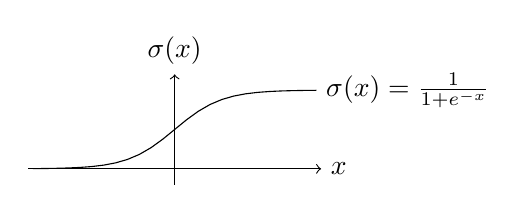
\begin{tikzpicture}[domain=-6:6,xscale=0.3]
  \draw[->] (-6.2,0) -- (6.2,0) node[right] {$x$};
  \draw[->] (0,-0.2) -- (0,1.2) node[above] {$\sigma(x)$};
  \draw plot (\x,{1 / (1 + exp(-\x))}) node[right] {$\sigma(x) = {1 \over 1 + e^{-x}}$};
\end{tikzpicture}
\caption{A sigmoidal (soft step) function.}
\label{fig:sigmoid}
\end{figure}

A number of variations for sigmoidal activation functions exist such as the 
hyperbolic tangent ($tanh$) and
the rectified linear unit \index{ReLU} (ReLU, see equation \ref{eq:ReLU}). 
They are applied either in a feedforward or recurrent (cyclic) manner, where
the recurrent variant are forced to cope with temporal transformations to
terminate\footnote{It is possible to \textit{unfold} recurrent
networks to resemble the circular processes until a certain point, achieving
a similar effect to temporal signal transformation, see \cite{Mozer1995}.}
\cite{Schmidhuber2014}.

\begin{equation} \label{eq:ReLU}
f(x) = \begin{cases}
         0 & \text{if } x < 0 \\
	 x & \text{otherwise}
       \end{cases}
\end{equation}

\subsection{Third generation neural networks}
Constructing a network of neuron models essentially creates a non-linear
response to a given numerical vector \cite{Russel2007}.
This transformative view can be adopted to biological \gls{NN}, where
the data being transferred are no longer vectors, but discrete
\textit{spikes} of electrical current \cite[p. 32]{Dayan2001, Eliasmith2004}.
In this case the activation of a spike can be understood as a function
of the electric current to the neuron cell along with the cell weights,
similar to the weighted sum in equation \ref{eq:weightedsum}
\cite[p. 234]{Dayan2001}.

There is a temporal dimension to this because signals in biological 
networks arrive from multiple sources in parallel \cite{Eliasmith2004}.
Lapicque presented the first model of conductance over time in 1907,
dubbed the \textit{integrate-and-fire} model, because neurons essentially
integrate received current over time to determine whether they should fire 
\cite{Dayan2001, Eliasmith2004}.
This understanding is the foundation for the \textit{third} generation
neural networks, where the computations occur in spikes over time 
\cite{Maass1997}.
Lapicque's model has been elaborated in the \textit{leaky
integrate-and-fire} model, which introduces a numerical ``leak''
into the model, that acts as a \textit{weight} for the neuron integration
\cite{Eliasmith2004, Eliasmith2015}.

\subsubsection{Encoding and decoding in spiking neural networks}
To align the bitwise numerical representation with the neural spikes
it is necessary to encode and decode the signals.
Because of the temporal nature of spiking neural networks, probability
distributions are commonly used to describe 
Given a current for background firing rates
Assuming there are $n$ inputs to a neuron with $i$ bits of information,
an encoder


An example of a network is shown in 

\begin{figure}
\centering
\tikzset{%
  every neuron/.style={
    circle, draw, minimum size=0.5cm
  },
  neuron dots/.style={
    draw=none,
    scale=1.5,
    text height=0.3cm,
    execute at begin node=\color{black}$\vdots$
  }
}
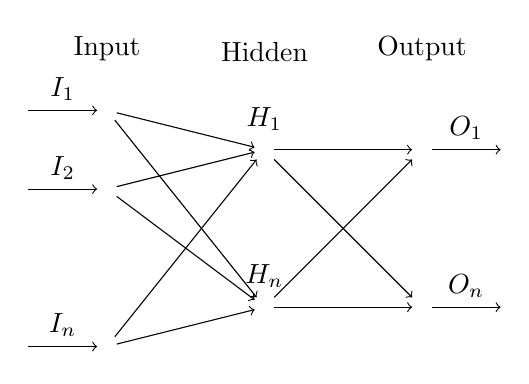
\begin{tikzpicture}{x=1.5cm, y=1.5cm}
  \foreach \m [count=\y] in {1,2,dots,n}
    \node [every neuron/.try, neuron \m/.try](input-\m) at (0, 2.5-\y) {};
  \foreach \m [count=\y] in {1, dots, n}
    \node [every neuron/.try, neuron \m/.try](hidden-\m) at (2, 2-\y) {};
  \foreach \m [count=\y] in {1, dots, n}
    \node [every neuron/.try, neuron \m/.try](output-\m) at (4, 2-\y) {};

  \foreach \l [count=\i] in {1, 2, n}
    \draw [<-] (input-\l) -- ++ (-1, 0)
      node [above, midway] {$I_{\l}$};
  \foreach \l [count=\i] in {1, n}
    \node [above] at (hidden-\l.north) {$H_{\l}$};

  \foreach \f in {1, 2, n}
    \foreach \t in {1, n}
      \draw [->] (input-\f) -- (hidden-\t);
  \foreach \f in {1, n}
    \foreach \t in {1, n}
      \draw [->] (hidden-\f) -- (output-\t);
  \foreach \l [count=\i] in {1,n}
    \draw [->] (output-\l) -- ++(1,0)
	node [above, midway] {$O_\l$};

  \foreach \l [count=\x from 0] in {Input, Hidden, Output}
    \node [align=center, above] at (\x*2,2) {\l};
\end{tikzpicture}
\caption{An example neural network with a single hidden layer.}
\label{fig:nn-example}
\end{figure}

circuits of computational
units connected through weighted edges \cite{Dayan2001, Eliasmith2004}.

% TODO: Distributions of properties instead of actual properties

% Both types of network are architecturally similar, and both are conceived from
% the same physiological principles \autocite{dayan2001, russel2007, Nilsson2009, schmidhuber2014}.
% The implementations, however, vary greatly.

% To ensure internal and external validity in and between the two network types,
% it is desirable that the models are as closely related from a theoretical and
% practical perspective as possible.
% Additionally, to test the hypothesis, it is required that both the artificial
% and spiking models can be simulated on regular machine architecture, while
% the spiking model requires a neuromorphic hardware platform.

% An optimal approach would be to find a tool that leverages the similarities
% of the network types, while integrating with the diverse simulated or emulated
% targets.
% That is, an abstract model of neural networks that can translate into
% heterogeneous back-ends, while retaining a high degree of inter-model validity.

% A number of general frameworks for artificial neural networks
% exist\footnote{
%   Among others, see \autocite{ONNX2018}, \autocite{PyTorch2018}, \autocite{TensorFlow2018},
%   \autocite{Keras2018} and DyNet \autocite{Neubig2017}.
% }, but none of them extend to the spiking domain.
% Conversely a number of choices exist for neuromorphic modelling\footnote{
%   %TODO: Find sources on internal IBM/Intel stuff
% }, but they exclusively evaluate to neuromorphic or spiking neural network
% backends \autocite{Jordan2018}.

\subsection{Learning in neural networks}


\subsubsection{Backpropagation}

\subsubsection{Auto-differentiation}
% TODO: Write about autodiff
\pagebreak
\section{Similar work}
A vast amount of work has been put into the development of software for simulating
neural networks.
This section covers the most popular and recent projects for both second and third
generation frameworks, and extracts relevant
features for use in the requirements section \ref{sec:requirements}.

\subsection{Second generation software}
The perhaps most noteable product for this type of networks is the Tensorflow \index{Tensorflow}
framework \cite{Abadi2016}.
Tensorflow is essentially an infrastructure for the description and execution of directed graph 
structures,
that connects varying activation functions and learning mechanisms through the common abstraction
of tensors \cite{Abadi2015}.
It is a large collaboration of multiple companies and organisations, who have
grown a comprehensive library of both code as well as infrastructure, and they
provide extensive hardware acceleration \cite{Abadi2015}.

The primary advantage of Tensorflow \index{Tensorflow} arrives from 
its foundation in tensors as a general abstraction that
can be applied to a wide array of problems \cite{Abadi2016}.
Other frameworks have adapted a similar approach, such as PyTorch \cite{PyTorch2018}, 
scikit-learn \cite{Sklearn2018}, Microsoft Cognitive Toolkit (CNTK) \cite{CNTK2018},
Caffe \cite{Caffe2018} and Theano \cite{Theano2018}.
The mentioned products differ slightly in terms of syntax and objective\footnote{Especially
PyTorch and Caffe targets \gls{DL}} as well as integrations for data and services, but
all rely on second generation \gls{NN} architecture.

Lasagne and Keras are examples of products that works with higher-level abstractions,
building on Theano and Tensorflow respectively \cite{Lasagne2018, Keras2018}.
They both provide imperative \gls{API}s for constructing models in steps, while
including useful utilities for the molding of data to fit the underlying tensor structures.

In terms of learning the frameworks are diverse, although gradient descent 
and auto-differentiation are among the most common features 
(seen in Tensorflow, PyTorch, CNTK, Theano
and Caffe). 
% TODO: Write about unsupervised/reinforcement learning?

The Open Neural Network Exchange Format (ONNX) is an open data format for the representation
of \gls{DL} learning models \cite{ONNX2018}. 
In this context ONNX is interesting because it attempts to describe the networks as 
a directed graph, just like Tensorflow.
ONNX is supported by Caffe, CNTK and Pytorch, and translate to Tensorflow,
indicating that a directed graph is 
sufficiently generic to model the structure and learning tasks within 
second generation networks.

\subsection{Third generation software}
The landscape for third generation software is less uniform, because the products target
wider applications.
In general 


PyNN is a simulator-independent

\section{DSL requirements} \label{sec:requirements}



\documentclass{report.tex}{subfiles}
\begin{document}
Before diving into the actual experiment built to test the hypothesis, this
chapter discusses and describes the method employed to model spiking
and artificial \gls{NN}s.

Both types of network are architecturally similar, and both are conceived from
the same physiological principles \autocite{dayan2001, russel2007, Nilsson2009, schmidhuber2014}.
The implementations, however, vary greatly.

To ensure internal and external validity in and between the two network types,
it is desirable that the models are as closely related from a theoretical and
practical perspective as possible.
Additionally, to test the hypothesis, it is required that both the artificial
and spiking models can be simulated on regular machine architecture, while
the spiking model requires a neuromorphic hardware platform.

An optimal approach would be to find a tool that leverages the similarities
of the network types, while integrating with the diverse simulated or emulated
targets.
That is, an abstract model of neural networks that can translate into
heterogeneous back-ends, while retaining a high degree of inter-model validity.

A number of general frameworks for artificial neural networks
exist\footnote{
  Among others, see \autocite{ONNX2018}, \autocite{PyTorch2018}, \autocite{TensorFlow2018},
  \autocite{Keras2018} and DyNet \autocite{Neubig2017}.
}, but none of them extend to the spiking domain.
Conversely a number of choices exist for neuromorphic modelling\footnote{
  %TODO: Find sources on internal IBM/Intel stuff
}, but they exclusively evaluate to neuromorphic or spiking neural network
backends \autocite{Jordan2018}.

A domain-specific language (DSL) called Volr was recently presented to
construct reproducible \gls{NN} experiments
\autocite{Pedersen2018:volr}.
The DSL allows the modelling of sufficiently complicated models for
the purpose of this thesis, while providing a set of tools that permits the
model be sent and evaluated on both \gls{ANN} and \gls{SNN} targets.

Some work was required to fully support learning mechanisms on
neuromorphic hardware, and the DSL, as well as the tooling around it, has been
extended for the purpose of this thesis (see appendix \ref{appendix:volr})
The following section describes the grammar and anatomy of Volr in detail.

\section{Volr}
Volr is a declarative DSL designed to model \gls{NN} that seeks a
trade-off between complete, but verbose, descriptions of small
networks and more general designs of large and complex networks.
By separating the network topologies from the detailed physiological properties
of each neuron or neuron population, the language aims to allow simple
experiments with few, concise declarations, as well as larger and more
complicated experiments while retaining readability.

Figure \ref{fig:volr-expr} shows the BNF form of expressions, values and types
in Volr, while figure \ref{fig:volr-rules} lists evaluation rules to apply
when evaluating the expressions.
Finally the \ref{fig:volr-examples} shows an example network that solves
a rudimentary maze task.
% Expressions, evaluation rules and examples
% Expression figure
\begin{figure}
  \begin{tabular}[t]{l l}
    expressions 
    & \texttt{$e$ ::= $n$} \\
    & \begin{minipage}{0.6\textwidth}
      \begin{Verbatim}[mathescape,commandchars=\\\{\}]
    | \textbf{stim} $n$
    | \textbf{pop} $n\ m$
    | \textbf{tar} $n$
    | $e \otimes e$
    | \textbf{let} $x = e$ \textbf{in} $e'$
      \end{Verbatim} 
    \end{minipage} \\
    & \\ % Empty space
    values
    & \texttt{$v$ ::= $n$} \\
    & \\ % Empty space

    types
    & \texttt{$\tau$ ::= \textbf{group} $n\ m$ | \textbf{stimt} $n$ | \textbf{int} }
  \end{tabular}

  \caption{Expressions, values and types of the Volr language.}
  \label{fig:volr-expr}
\end{figure}

\begin{figure}
\begin{prooftree}
  \AxiomC{}
  \RightLabel{\hskip10pt($e1$)}
  \UnaryInfC{$\Gamma \vdash n : \mathbf{int}$}
\end{prooftree}
\begin{prooftree}
  \AxiomC{}
  \RightLabel{\hskip10pt($e2$)}
  \UnaryInfC{$\Gamma \vdash \mathbf{stim}\ n : \mathbf{net}\ 1\ n$}
\end{prooftree}
\begin{prooftree}
  \AxiomC{}
  \RightLabel{\hskip10pt($e3$)}
  \UnaryInfC{$\Gamma \vdash \mathbf{pop}\ n : \mathbf{net}\ 1\ n$}
\end{prooftree}
\begin{prooftree}
  \AxiomC{$\Gamma (x) = \tau$}
  \RightLabel{\hskip10pt($e4$)}
  \UnaryInfC{$\Gamma \vdash x : \tau$}
\end{prooftree}
\begin{prooftree}
  \AxiomC{$\Gamma \vdash e_1 : \mathbf{net}\ l\ m$}
  \AxiomC{$\Gamma \vdash e_2 : \mathbf{net}\ n\ q$}
  \AxiomC{$\Gamma \vdash w : \mathbf{float}$}
  \RightLabel{\hskip10pt($e5$)}
  \TrinaryInfC{$\Gamma \vdash \otimes\ e_1\ e_2\ w : \mathbf{net}\ l\ q$}
\end{prooftree}
\begin{prooftree}
  \AxiomC{$\Gamma \vdash e_1 : \mathbf{net}\ l\ m$}
  \AxiomC{$\Gamma \vdash e_2 : \mathbf{net}\ m\ n$}
  \AxiomC{$\Gamma \vdash w : \mathbf{float}$}
  \RightLabel{\hskip10pt($e6$)}
  \TrinaryInfC{$\Gamma \vdash \ominus\ e_1\ e_2\ w : \mathbf{net}\ l\ n$}
\end{prooftree}
\begin{prooftree}
  \AxiomC{$\Gamma \vdash e : \tau$}
  \AxiomC{$\Gamma [v : \tau] \vdash e' : \tau$}
  \RightLabel{\hskip10pt($e7$)}
  \BinaryInfC{$\Gamma \vdash \mathbf{let}\ x = e\ in\ e' : \tau$}
\end{prooftree}

  \caption{Evaluation rules in Volr.}
  \label{fig:volr-rules}
\end{figure}



\begin{figure}
  \ContinuedFloat*
  \begin{tabular}[t]{l c}
    \begin{minipage}{0.4\textwidth}
      \begin{Verbatim}[mathescape,commandchars=\\\{\}]
\textbf{dense} 2 2
      \end{Verbatim}
    \end{minipage} & \begin{minipage}{0.4\textwidth}
      \includegraphics[width=\textwidth]{chapters/volr/example2.pdf}
    \end{minipage}

  \end{tabular}
  \caption{A network with a stimulus containing two channels.
    The stimulus is fully connected to a population with an excitatory
    weight of 1. Each circular node represents a single neuron.}
  \label{fig:volr-example1}
\end{figure}

\begin{figure}
  \ContinuedFloat
  \begin{tabular}[t]{l c}
    \begin{minipage}{0.4\textwidth}
      \begin{Verbatim}[mathescape,commandchars=\\\{\}]
\textbf{let} s$_1$ = \textbf{dense} 1 1 \textbf{in}
\textbf{let} s$_2$ = $\neg$ \textbf{dense} 1 1 \textbf{in}
(s$_1$ $\ominus$ s$_2$) $\obar$ \textbf{dense} 2 1
      \end{Verbatim}
    \end{minipage} & \begin{minipage}{0.6\textwidth}
      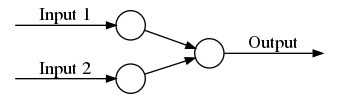
\includegraphics[width=\textwidth]{chapters/volr/example1.pdf}
    \end{minipage}
  \end{tabular}
  \caption{An illustration of a simple binary network, whose two 
	   parallel layers share the middle population of size 2.}
\end{figure}

\begin{figure}
  \ContinuedFloat
  \begin{tabular}[t]{l c}
    \begin{minipage}[b]{0.4\textwidth}
      \begin{Verbatim}[mathescape,commandchars=\\\{\}]
      \textbf{dense} 100 50
        $\obar$ \textbf{dense} 50 10
      \end{Verbatim}
    \end{minipage} & \begin{minipage}{0.5\textwidth}
      \includegraphics[width=\textwidth]{chapters/volr/example3.pdf}
    \end{minipage}
  \end{tabular}
  \caption{A larger network that can process the MNIST dataset
    as 10x10 pixel images. 
    The nodes are populations of neurons,
    where the input corresponds to the pixel size ($10\cdot10=100$) 
    and the output to the possible classes (0 - 9).
    Input and output are implicit.}
\end{figure}

\begin{figure}
  \begin{tabular}[t]{l c}
    \begin{minipage}{0.45\textwidth}
      \begin{Verbatim}[mathescape,commandchars=\\\{\}]
\textbf{let} s = \textbf{dense} 2 2 \textbf{in}
\textbf{let} l$_1$ = \textbf{dense} 2 4 \textbf{in}
\textbf{let} l$_2$ = \textbf{dense} 2 4 \textbf{in}
\textbf{let} o = \textbf{dense} 8 1 \textbf{in} 
  s $\obar$ (l$_1$ $\ominus$ l$_2$) $\obar$ o
      \end{Verbatim}
    \end{minipage} & \begin{minipage}{0.5\textwidth}
       \includegraphics[width=\textwidth]{chapters/volr/example4.pdf}
    \end{minipage}
  \end{tabular}
   \caption{An example where a two-dimensional input is split into
     two nodes and later merged into a node of a single neuron.}
  \label{fig:volr-examples}
\end{figure}



\newpage\null\thispagestyle{empty}\newpage
\newpage\null\thispagestyle{empty}\newpage
\pagebreak
Figure \ref{fig:volr-bnf} shows the constituent parts of an experiment.
Four sub-com\-po\-nents are required:
  A number of stimuli, neural populations, responses and experiment targets.

\subsubsection{Block grammar} \label{sec:volr-block}
The sub-components are constructed using the same declarative \textit{block}
structure shown in figure \ref{fig:volr-ebnf-block}.
The block defines its \textit{type} (\texttt{stimulus}, \texttt{population},
\texttt{response} or \texttt{target}), an optional \textit{name} and lastly
some block content.

The content varies for the different block types, but is restricted to contain
a number of either key-value pairs (\texttt{field}s) or relations to other
blocks (\texttt{connection}s).
Fields are interpreted by the respective targets (see section
\ref{sec:volr-targets}) and connections are only allowed for
\texttt{population}s and \texttt{responses}.

\subsubsection{Connection-set algebra grammar} \label{sec:volr-csa}
Connections between blocks are implemented as a subset of the \gls{CSA}
introduced in section \ref{sec:CSA} \autocite{Djurfeldt2012}.
Most notably, the notion of \textit{blocks} and \textit{geometric distance} have
been omitted\footnote{Neither blocks nor distances are required for the
  experiment in the thesis. It is, however, a necessary element to conduct
  further experiments, since biological \gls{SNN} are highly influenced by
  spatial arrangements \autocite{dayan2001}.
}.

The grammar is presented in figure \ref{fig:volr-ebnf-csa}, and aims to provide
a flexible way to describe complex connectivity patterns in text.
The present grammar can be viewed as a basic algebraic tool for set operations.
Describing full connectivity between two populations, such that all neurons
in the first population is connected with all neurons in the second population,
can simply be expressed as `\texttt{all}'.
Connecting one neuron to one other neuron between two populations are described
as `\texttt{one}', while random connectivity are described with a probability
of, say 0.5: `\texttt{random 0.5}'\footnote{
  This expresses a Bernouilli trial with the given probability
  \autocite{Djurfeldt2012}.
}
As a final example, every neuron in a population connected to every neuron in
that same population, with the exception of identical neurons, can be described
as `\texttt{all - self}'.
%
% \begin{figure}
%   \begin{center}
%     \begin{minipage}{0.8\linewidth}
%       \begin{grammar}
%         <connection> ::= 'from' , <block-name> , { <csa-expr> } ;
%
%         <csa-expr> ::= <csa-term> | <csa-expr> , <csa-operator> , <csa-expr> ;
%
%         <csa-term> ::= 'all' | 'one' | 'self' | 'random' , <number> ;
%
%         <csa-operator> ::= '+' | '-' | '*' ;
%       \end{grammar}
%     \end{minipage}
%   \end{center}
%   \caption{BNF of the connection grammar, describing relations between
%     blocks through \gls{CSA}.}
%   \label{fig:volr-bnf-csa}
% \end{figure}

\subsubsection{Experiment stimuli}
The stimuli describes the ``input'' of the model.
Such input is defined either as an array of elements directly in the DSL
or as a reference to a file.

\subsubsection{Experiment populations}
The populations describe the topology of the neural network itself.
As with the stimuli, the populations are built around a block structure that
contains a number of sub-expressions.

The \texttt{connection} defines the source stimulus for the population,
i.e. the population \textit{from} which action-potentials will be forwarded.
A population can receive stimulus from more than one source.
The connections are modelled as per the \gls{CSA} described in section
\ref{sec:volr-csa}.

% TODO: Describe and invent archetypes... or not?

\subsubsection{Experiment responses}
The responses are the ``output'' of the model to be recorded, and can be
considered as the outcome of the network for training purposes.
The response block only contains an optional specification of a location for
the experiment output data.

\subsubsection{Experiment targets}
The final element in a Volr experiment is its targets.
A target describe a destination environments on which to run the experiment.
These are described in detail in section \ref{sec:volr-targets}, and are
referenced in the grammar as simple strings.

\subsection{Volr semantics}
In practice a network is built by describing a graph.
The nodes in the graph consist of \texttt{populations} of neurons and the edges
are connection-set matrices to other populations \autocite{Djurfeldt2012}.
% TODO: Describe CSA
\texttt{Populations} can consist of any positive number of neurons and is
required to have at least one connection.
Connections can be recursive, resulting in a potentially cyclic graph.
Both the connections and the \texttt{populations} can be annotated with features
such as connection weight and neuron parameters (see \nameref{appendix:volr}).
The parameters are treated differently depending on the experiment target (see
sections \ref{sec:volr-NEST} and \ref{sec:volr-BrainScaleS}).


\section{Neural network simulation targets in Volr} \label{sec:volr-targets}

% TODO :Write how fields are interpreted
% TODO: Write how input is interpreted

Volr exploits the structural similarities between \gls{ANN} and \gls{SNN} to
translate the model to both spiking and artificial network platforms (back-ends).

In the remainder of the chapter the three emulation back-ends, shown in figure
\ref{fig:volr}, are described:
a machine learning target for \gls{ANN}s and a neuron simulation target, as well
as a neuromorphic hardware target, for \gls{SNN}s.

\begin{figure}
  \centering
  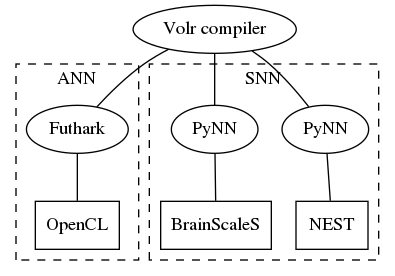
\includegraphics[width=0.6\textwidth]{images/volr-architecture.png}
  \caption{The translation from the Volr DSL to \gls{ANN} simulations in OpenCL via
    \gls{Futhark} and to \gls{SNN} simulations on \gls{NEST} and \gls{BrainScaleS}
    via the \gls{Myelin} middleware.
  }
  \label{fig:volr}
\end{figure}

\subsection{Translation to Futhark} \label{sec:volr-futhark}
Futhark is a functional data-parallel programming language \autocite{Henriksen2017}.
It offers a number of compilation targets such as \gls{OpenCL}, which is
particularly interesting for this thesis because of its capacity for hardware
acceleration.

The practical translation from the Volr model to Futhark is built on recurrent
\gls{ANN} with stochastic gradient descent backpropagation
\autocite{russel2007, schmidhuber2014}.
Each neuron population is considered as a single layer, whose connections are
determined by a connection matrix.

% Deal with recurrent connections
% Describe how this relates to layers

... To be continued ...

\subsection{Spiking neural network simulations via PyNN} \label{sec:volr-pynn}
The Python neural network simulation interface PyNN is designed as a
"simulator-independent language for building neuronal network models"
\autocite{PyNN2018}.
It aims to reduce the problem of diverse, and occasionally unique, descriptions
of neural network experiments for different simulation back-ends \autocite{Davison2009}.
PyNN has been adapted by a number of simulators, including the NEST simulation
platform and the neuromorphic BrainScaleS wafer system
\autocite{Davison2009, Helias2012, Schmitt2017}.

There are still simulator-dependent configurations that seems unlikely to be
adopted into PyNN in the immediate future\footnote{
  Particularly hardware mapping configurations are hard to abstract in a general
  interface.
}.
For that reason Volr provides simulation-specific PyNN scripts that can
interpret the model in the context of each simulation target.
A middleware, dubbed \gls{Myelin}, was invented to translate the \gls{NN} model
into a static intermediate representation in JSON.
The JSON standard was chosen for the task because of its concise syntax while
still retaining human readability.

The advantage of the static experiment representation being, that the experiment
easily a) transports to the target PyNN scripts without losing any information,
and b) duplexes between several experiment; the same experiment setup is
trivial to setup on multiple targets at once.

The correct execution of the experiments relies on the PyNN scripts to exploit
the simulator to represent the Volr model as accurately as possible.
Fortunately PyNN is designed to cover exactly such a use case, so properties
related to the \gls{NN} models itself (such as network topology and population
attributes) were faithfully reproduced across the simulators.
However, the simulators deviate in a number of ways that are relevant to
mention.
The following two sections explains the steps necessary to achieve accurate
experiment environments in \gls{NEST} and \gls{BrainScaleS}.

\subsubsection{Translation to PyNN} \label{sec:volr-translation}

\subsubsection{Translation to NEST} \label{sec:volr-NEST}
... To be continued ...
\subsubsection{Translation to BrainScaleS} \label{sec:volr-BrainScaleS}
... To be continued ...
\end{document}
\end{document}
